\documentclass[../Head/Main.tex]{subfiles}
\begin{document}
\begin{figure}[H]
	\centering
		\begin{tikzpicture}
		\node[anchor=south west, inner sep=0] (image) at (0,0) {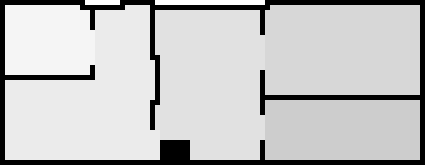
\includegraphics[width=0.65\textwidth]{Maps/map_5_rooms}};
		\node[align=center, black, font={\large}] at (1.25,3.25) {Room 1};
		\node[align=center, black, font={\large}] at (2,1.25) {Room 2};
		\node[align=center, black, font={\large}] at (5.45,2.25) {Room 3};
		\node[align=center, black, font={\large}] at (9,3) {Room 4};
		\node[align=center, black, font={\large}] at (9,0.9) {Room 5};
		\end{tikzpicture}		
	\caption{Illustration of "5-room world"}
	\label{fig:5_room_world}
\end{figure}
\end{document}